%%% MATERIALS AND METHODS %%%


\subsection*{Carbon Fiber Filament}

To print carbon fiber a novel CFRP filament was developed using a 1K carbon fiber tow with ABS plastic as the matrix material. Two production methods were explored for creating this filament. First, a pultrusion technique which combined a standard ABS FDM filament and carbon fiber using a 3Doodler, a handheld FDM printer, was attempted. Experimentation with dipping the tow through an ABS-acetone slurry was also explored.

\begin{figure}[t]
        \centering
        \begin{subfigure}[b]{0.4\linewidth}
                \includegraphics[width=\linewidth]{./figures/pultrusion-vid}
                \caption{Pultrusion.}
                \label{fig:pultrusion-vid}
        \end{subfigure}
        \begin{subfigure}[b]{0.4\linewidth}
                \includegraphics[width=\linewidth]{./figures/dipping-vid}
                \caption{Dipping.}
                \label{fig:dipping-vid}
        \end{subfigure}
        \caption{CFRP production methods.}\label{fig:slurry-making}
\end{figure}

Pultrusion experiments quickly demonstrated this method's failure to achieve wet-out of the entire tow. Subsequently, all CFRP development methods were shifted to dipping configurations. A viable CFRP filament was attempted to be created by altering the ABS concentration in ABS-acetone slurries and then quantifying the physical and mechanical properties of the filaments. ABS concentrations by volume ranging from 9\% to 16\% were experimented with and filament diameter, tow center, frequency of defects were considered for determining the optimal method. Figure~\ref{fig:filament-microscope} shows a micrsocope image of a sample filament, approximately 1.5 mm in diameter.

\begin{figure}[t]
        \centering
        \begin{subfigure}[b]{0.4\linewidth}
                \includegraphics[width=\linewidth]{./figures/filament-108-40-dip-side}
                \caption{Length.}
                \label{fig:filament-108-40-dip-side}
        \end{subfigure}
        \begin{subfigure}[b]{0.4\linewidth}
                \includegraphics[width=\linewidth]{./figures/filament-108-40-dip-end}
                \caption{Cross section.}
                \label{fig:filament-108-40-dip-end}
        \end{subfigure}
        \caption{Microscopic photos (10X) of a CFRP filament created with 10 dips in a 16\% ABS solution.}\label{fig:filament-microscope}
\end{figure}

%\begin{figure}[t]
%        \centering
%        \begin{subfigure}[b]{0.3\linewidth}
%                \includegraphics[width=\linewidth{./figures/filament-108-40-dip-side}
%                \caption{Length.}
%                \label{fig:filament-108-40-dip-side}
%        \end{subfigure}
%        \begin{subfigure}[b]{0.3\linewidth}
%                \includegraphics[width=\linewidth]{./figures/filament-108-40-dip-end}
%                \caption{Cross section.}
%                \label{fig:filament-108-40-dip-end}
%        \end{subfigure}
%        \caption{Microscopic photos (10X) of a CFRP filament created with 10 dips using the fully immersed guide in a 16\% ABS solution.}\label{fig:filament-microscope}
%\end{figure}

\subsection*{Extruder Design}

An FDM extruder end-effector was designed and fabricated for the curved layer carbon fiber 3D printer. The extruder is the mechanism responsible for depositing the CFRP filament, which is accomplished by reeling in the filament, heating, and printing it. For mounting to the FANUC robot, the extruder's prime design constraints were to includes attachment fixtures for connecting to the robot's Schunk pneumatic gripper and use geometries and materials that minimize torque on the gripper jaws. The designed extruder uses RepRap 3D printing hardware and custom components (machined aluminum and laser-cut acrylic). To drive the filament into the heating chamber, a notched screw, which rests on two bearings, receives a 3:1 step-up in torque from a stepper motor. A bearing for filament counterpressure is mounted between an adjacent set of carrier plates, which can be translated to accomodate filament sizes ranging from 1.75 to 3 mm. Figure~\ref{fig:extruder-side-profile} shows an image of the fabricated extruder, which was designed in SolidWorks, pulling and and printing filament.

%\begin{figure}[htp]
%\centering
%\includegraphics[width=0.8\linewidth]{./figures/extruder-iso}
%\caption{A SolidWorks rendering of the extruder.}
%\label{fig:extruder-iso}
%\end{figure}

\begin{figure}[htp]
\centering
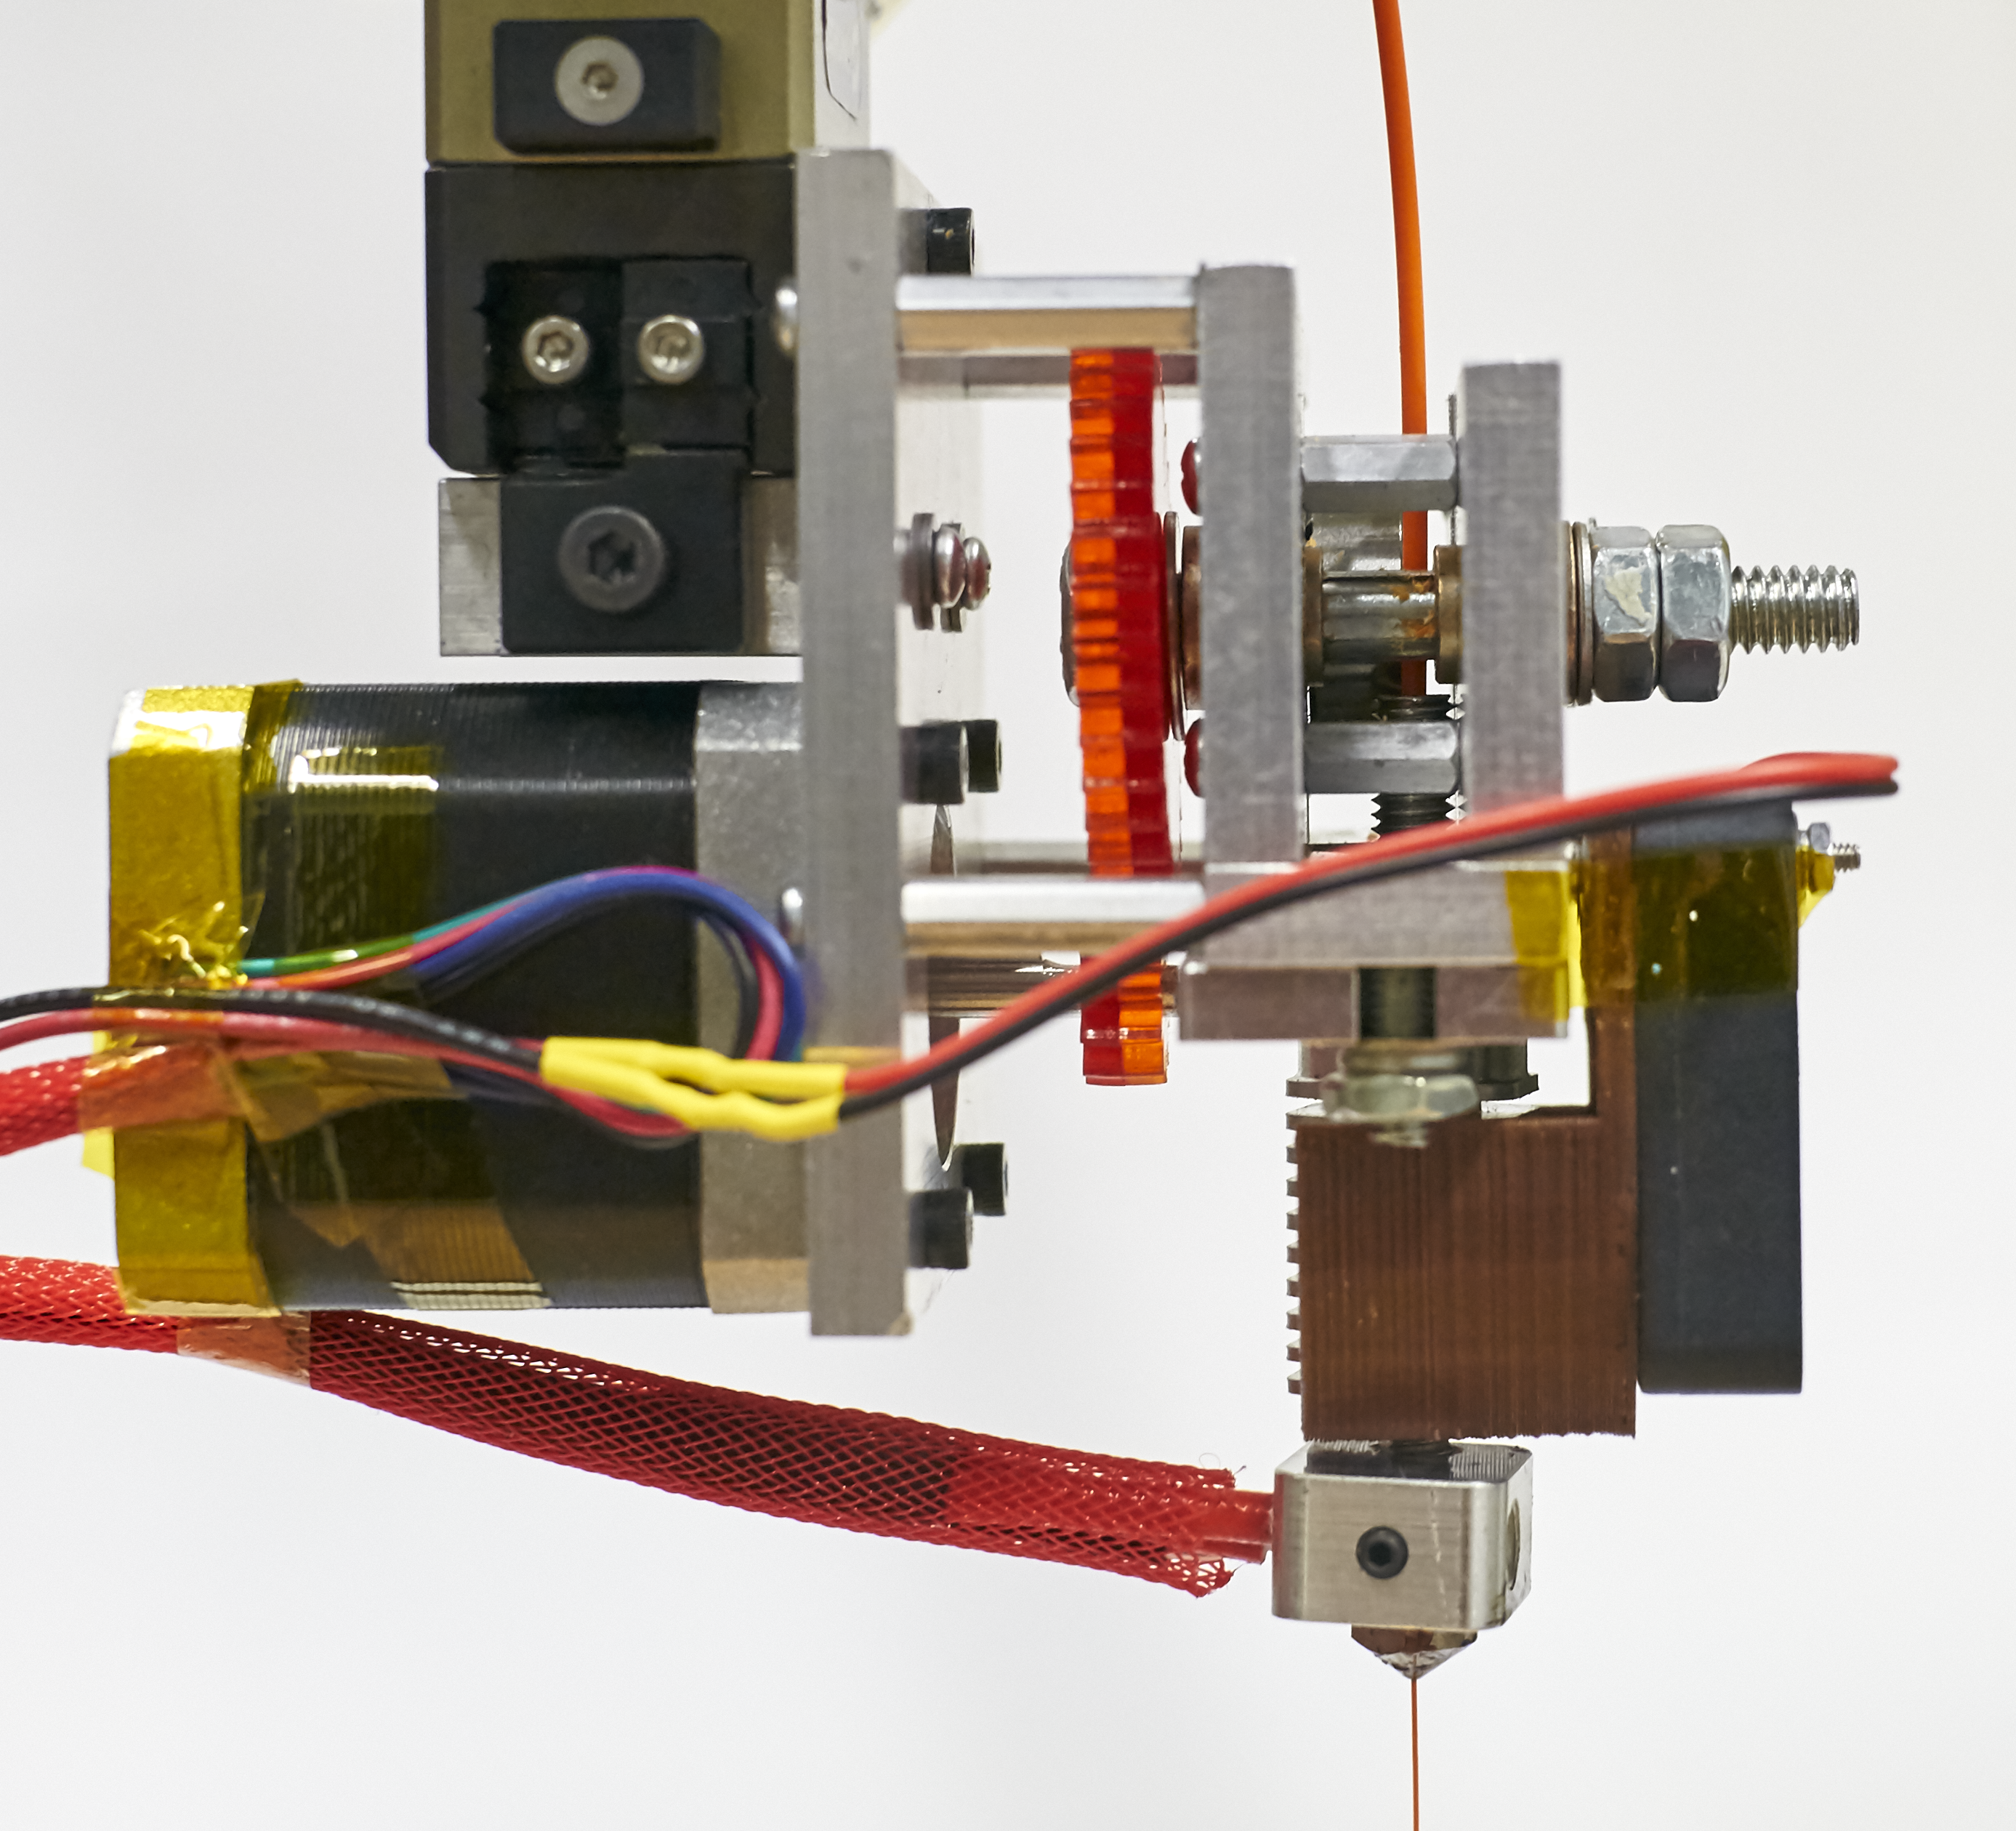
\includegraphics[width=0.8\linewidth]{./figures/extruder-side-profile}
\caption{A photo of the side profile of the built extruder.}
\label{fig:extruder-side-profile}
\end{figure}

%test text\\

\subsection*{Finite Element Analysis}

ANSYS Composite PrepPost (ACP) finite element analysis software was used to predict the mechanical properties and failure behavior of the bridge specimen. ACP utilizes orthopic shell elements, ply thickness assignments, oriented element sets, and stackup configurations to model and analyze fiberous, composite structures of multiple layers. A surface representation of the bridge specimen, shown in Figure~\ref{fig:fea-bridge-speciment}, was modeled in SolidWorks and imported in ACP. Material properties for ABS and carbon fiber were used in their respective directions to define the orthotropic elements.

Various failure criteria, such as Puck or Tsai-Wu failure theories, can be utilized in ACP to predict failure modes and critical layers given the applied loads and boundary conditions \cite{ACP-manual}. Puck's failure criterion, a phenomenological failure behavior for uni-directional (UD) CFRPs \cite{Puck-Stuttgard,Puck-NASA}, was applied to this model under the loading conditions desribed in the introduction. This mimics the printing condition where all printed CFRP strands are extruded lengthwise so that the carbon fibers react most of the tesile bending stresses caused by compression of the part ends. Figure~\ref{fig:fea-acp-asme} shows the ACP representation of the model, which utilizes a layer thickness 0.4 mm (the extruder end-effector nozzle outlet diameter) to achieve a desired part thickness of 3.175 m.

\begin{figure}[htp]
\centering
\includegraphics[width=0.8\linewidth]{./figures/fea/fea-surface-geometry}
\caption{The surface geometry used in ACP.}
\label{fig:fea-bridge-speciment}
\end{figure}

\begin{figure}[htp]
\centering
\includegraphics[width=0.8\linewidth]{./figures/fea/fea-acp-asme}
\caption{ACP FEM showing fiber direction and layers.}
\label{fig:fea-acp-asme}
\end{figure}

%test text. test citations \cite{Puck-Stuttgard,Puck-NASA}.\\

\subsection*{Print Controls}

Typical FDM 3D printers, including industrial, home, and do-it-yourself printers, use a Cartesian-style gantry system with 3 degrees of freedom. Such printers can achieve some degree of curved-layer printing, but the fixed print head attitude limits the curved-layer geometries to those accessible from one approach angle. To remove this limitation, a 6-degree-of-freedom FANUC LR Mate 200iC robotic arm was used for this project. The robot provides a similar resolution and repeatibility to other FDM printers, with a somewhat larger build envelope, making it a good candidate to become an FDM printer platform. Some of the remaining elements of the printer control system were chosen from existing open-source hardware and software from the RepRap community, while others were chosen from FANUC products.

Figure~\ref{fig:sys-overview} gives a schematic overview of the mechanical, hardware, and software components that make up the curved-layer 3D printer system. The robot arm is the mechanical platform for the 3D printer. The custom extruder is fitted to the end of the robot arm and acts as a printing end effector. The motion of the robot arm is controlled by the robot controller, which is programmed by writing TP programs via the controller teach pendant. The extruder hardware, including the heater cartridge, cooling fan, and extrusion motor are controlled by an open-source Megatronics board loaded with the (also open-source) Marlin firmware. 

In a typical RepRap 3D printer using a Megatronics board, the Megatronics board is used to control the path of the extruder as well as the extrusion feed rate; the Marlin firmware can adjust the extruder filament feedrate according to the surface speed of the extruder in order to maintain the desired volu. However, here, the FANUC controller provides the motion control, while the Megatronics board only controls the extrusion. Thus, additional interfacing is required to provide the Megatronics board with real-time information about the robot's motion. For this purpose, I/O hardware was connected to the FANUC robot controller. The I/O hardware was installed in a purpose-built cabinet and installed near the FANUC controller, shown in Figure~\ref{fig:cabinet-2}. During motion, an analog output from the I/O module provides the extruder surface speed to the Megatronics board, which can use that information to control the extrusion speed accordingly.

The Megatronics board was chosen for its easy setup and campatibility with other widely-used 3D printing hardware and software, including the Marlin firmware. Once configured for the Megatronics board and for filament drive geometry of the custom extruder, the firmware was uploaded using the popular Arduino IDE. The board was mounted on the robot cage frame for easy access during debugging and maintenance and for proximity to the printing area, shown in Figure~\ref{fig:mounted-mega}. The Megatronics board receives G code commands from a connected computer over a USB interface from the Pronterface program, which provides a graphical interface for common 3D printer controls. 

\begin{figure}[t]
    \centering
    \includegraphics[width=.8\linewidth]{figures/mounted-mega}
    \caption{The mounted Megatronics board.}
    \label{fig:mounted-mega}
\end{figure}

\begin{figure}[t]
    \centering
    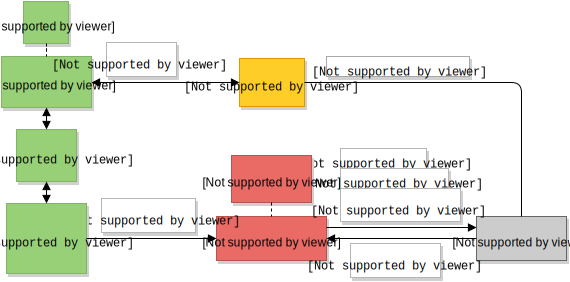
\includegraphics[width=.8\linewidth]{figures/diagrams/system overview}
    \caption{Overview of the 3D printer controls.}
    \label{fig:sys-overview}
\end{figure}

\begin{figure}[t]
    \centering
    \includegraphics[width=.8\linewidth]{figures/cabinet2}
    \caption{The I/O cabinet installed alongside the FANUC controller.}
    \label{fig:cabinet-2}
\end{figure}

\subsection*{FANUC Setup}

The FANUC robot required some setup and programming to be used as an FDM 3D printing platform. New coordinate frames were defined in the robot system to facilitate the later creation of motion instructions. One of these frames is the User Frame, which is attached to the bed of the robot cage, and does not move with the robot; this frame is used as the 3D printing frame. The other frame is the Tool Frame, which is attached to the tip of the custom extruder nozzle and moves with the end of the robot arm. The frame allows motion instructions to be written that moves the nozzle tip precisely without extra calculations. The frames were defined using built-in procedures on the robot controller.

A TP (Teach Pendant) program was writted to generate the printing toolpath for the curved-layer test specimen used in the FEA studies for this project. In other 3D printing systems, the desired 3D model is "sliced", and the resulting toolpath is sent to the printer controller as G-code. Because the FANUC controller does not accept G-code, its built in TP language was used. Because TP must be manually written unless external FANUC software is used, the curved-layer specimen geometry was chosen to be created with minimal TP motion instructions. 

An additional TP program was written to generate the analog output signal to send the speed of the nozzle tip to the Megatronics board. This program was set as a Background Logic program, which the FANUC controller runs every 4ms regardless of what other programs are currently running. 
